\textcolor{secundario}{\textbf{\textit{PEERS Valuation}.}}\\[5pt]

The appraiser applied the methodology known as Relative Valuation, using the models known as Trading Multiples and/or  M\&A Transaction Multiples, in accordance with the market approach.\\




%\begin{figure}
%\caption{Modelo de Valuaci\'on Relativa.\label{fig:peers1}}
%
\includegraphics[width=8cm]{\rutaImagenes/peers_1}
%\end{figure}
%
%\begin{figure}
%\caption{PEERS m\'as Utilizados.\label{fig:peers2}}
%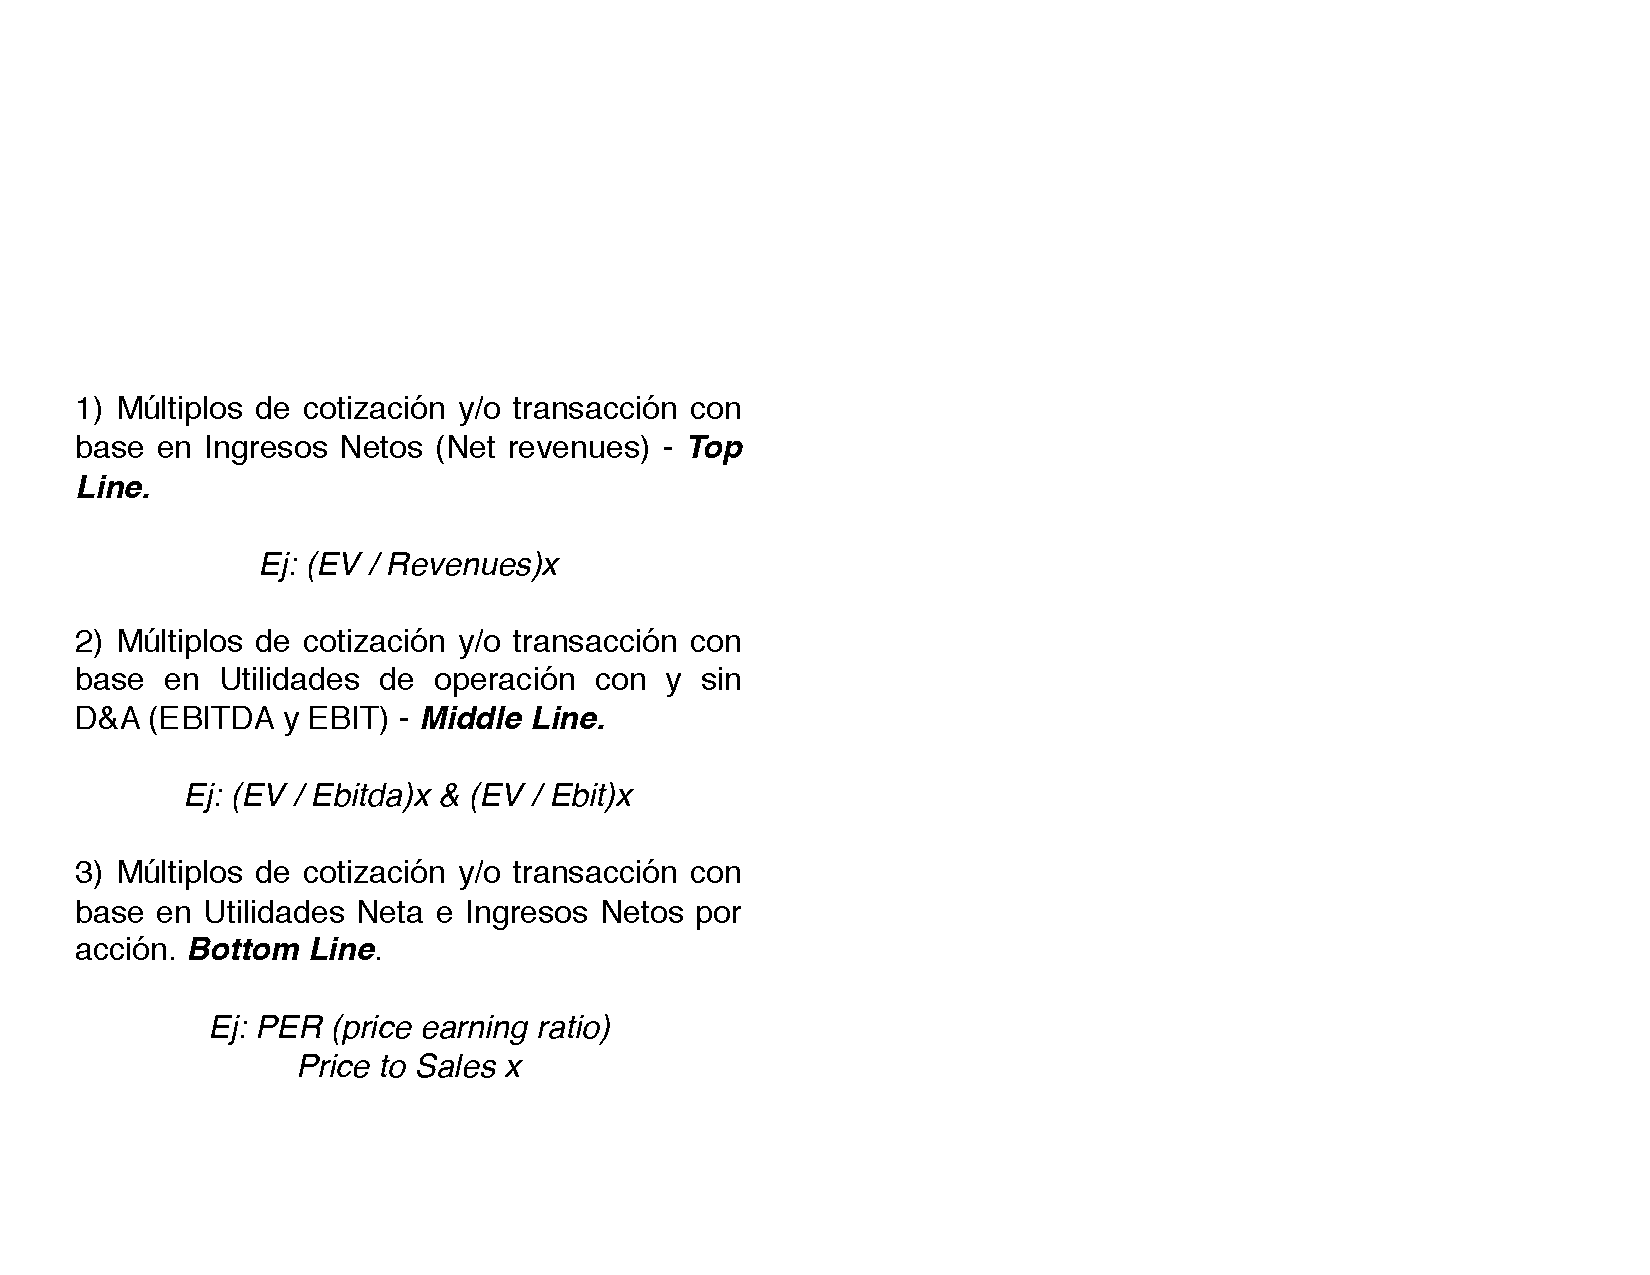
\includegraphics[width=8cm]{\rutaImagenes/peers_2}
%
%\end{figure}
\begin{figure}[H]
\caption{Relative Valuation Model. Most Commonly Used PEERS\label{fig:peers1}}\vspace{5pt}
 \raisebox{-0.5\height}{
\includegraphics[width=6cm]{\rutaImagenes/peers_1}}
       \hfill
       \raisebox{-0.5\height}{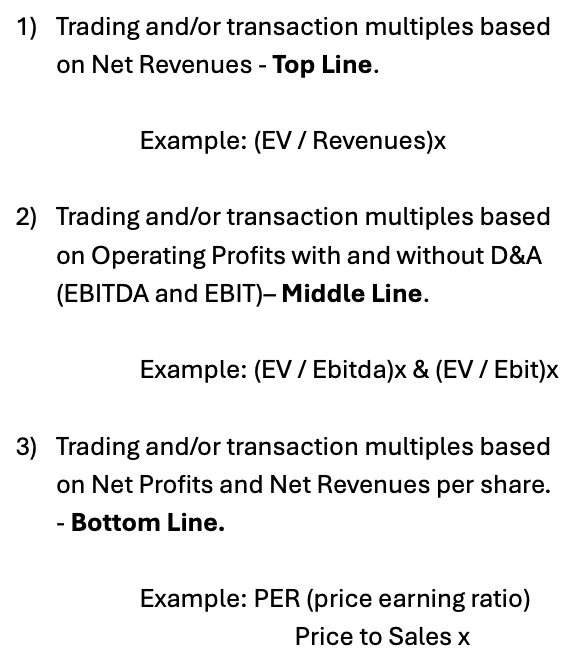
\includegraphics[width=6cm]{\rutaImagenes/peers_2_eng}}
\end{figure}

 
 This methodology allows for the determination of the value of companies not listed on the stock market, and in the case where the company being valued is listed, the method can help detect whether the market is over or undervaluing the asset in question. Furthermore, it enables the determination of the \textit{\gls{marketaproach}} component in a financial valuation, using a representative sample on the ideal multiple for the subject of valuation.\\

 